\documentclass[12pt]{llncs}

\usepackage[utf8]{inputenc}
\usepackage[T1]{fontenc}
\usepackage{amsmath}
\usepackage{amssymb}
\usepackage{mathtools}
\usepackage{parskip}
\usepackage{tikz}
\usepackage{subcaption}

\usetikzlibrary{arrows}

\captionsetup{compatibility=false}

\DeclarePairedDelimiter{\set}{\{}{\}}
\DeclarePairedDelimiter{\tuple}{(}{)}
\DeclarePairedDelimiter{\abs}{\lvert}{\rvert}

\let\oldleq\leq
\renewcommand{\leq}[1][]{\oldleq_{#1}}
\renewcommand{\implies}{\rightarrow}

\newcommand{\bicond}{\leftrightarrow}
\newcommand{\poset}[1]{\mathcal{#1}}
\newcommand{\uni}[1][]{\Omega_{#1}}
\newcommand{\lang}[1]{L(#1)}
\newcommand{\lin}[1]{\texttt{#1}}
\newcommand{\swap}[1][]{\leftrightarrow_{#1}}
\newcommand{\sgraph}[1]{G(#1)}
\newcommand{\lext}{\sqsubseteq}
\newcommand{\incomp}{\parallel}
\newcommand{\covered}{\prec}
\newcommand{\complmt}[1]{\overline{#1}}
\newcommand{\satvar}[2]{\mathtt{X}_{#1}^{#2}}
\newcommand{\bigo}[1]{\mathcal{O}(#1)}

\begin{document}

\title{Poset Paper}
\author{Bow-yaw Wang\inst{1} \and Chih-chen Yuan\inst{2}}
\institute{Academia Sinica, Taiwan\\ \and
National Taiwan Normal University, Taiwan}
\maketitle

\begin{abstract}
hello world
\end{abstract}

\section{Introduction}
Intro part here

\section{Preliminaries}
A \emph{partial order} is a binary relation that is reflexive, antisymmetric, and transitive. A partially ordered set or poset is a binary structure $\poset{P} = \tuple{\uni, \leq}$ where the \emph{universe} $\uni$ is a set and $\leq$ is a partial order on $\uni$; we refer to members of $\uni$ as elements of $\poset{P}$ and, where specificity is desired, to $\uni$ as $\uni[
\poset{P}]$ and $\leq$ as $\leq[\poset{P}]$.

% example:posetp
\begin{example}
    For the following definition, consider the poset $\poset{P}$ over $\set{a,b,c,d}$ with $a \leq b$; $a \leq c$; $a \leq d$; $b \leq d$; and $c \leq d$. Figure~\ref{figure:posetp} describes $\poset{P}$ with a graph $\tuple{V,E} = \tuple{\Omega,\covered}$.
    \label{example:posetp}
\end{example}

% figure:posetp
\begin{figure}
    \centering
    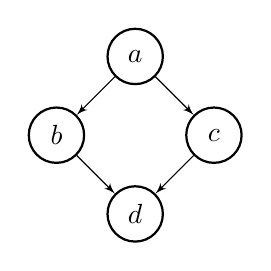
\begin{tikzpicture}
        [
        vertex/.style={circle,thick,draw,minimum size=2em},
        edge/.style={->,> = latex'}
        ]
    \node[vertex] (1) at (1,2) {$a$};
    \node[vertex] (2) at (0,1) {$b$};
    \node[vertex] (3) at (2,1) {$c$};
    \node[vertex] (4) at (1,0) {$d$};
    \draw[edge] (1) -- (2);
    \draw[edge] (1) -- (3);
    \draw[edge] (2) -- (4);
    \draw[edge] (3) -- (4);
    \end{tikzpicture}
    \caption{Graph representation of $\poset{P}$ from Example~\ref{example:posetp}.}
    \label{figure:posetp}
\end{figure}

The \emph{cover} relation $\covered$ of a poset $\poset{P}$ is the transitive reduction of the order relation; it describes the case of immediate successor: for $x, y \in \poset{P}$, $x \covered y$ iff $x \leq y \wedge \not\exists z \in \poset{P}, x \leq z \wedge z \leq y$. For Example~\ref{example:posetp}, the covered relation includes $a \covered b$; $a \covered c$; $b \covered d$; and $c \covered d$. Note that $\tuple{a,d}$ is absent in $\covered$.

In addition, we describe the case of \emph{incomparability} in a poset $\poset{P}$ with $\incomp$: for $x, y \in \poset{P}$, $x \incomp y$ iff $x \not\leq y \wedge y \not\leq x$. For Example~\ref{example:posetp}, there is $b \incomp c$.

% example:posetl
\begin{example}
    For the following definition, consider the poset $\poset{L}$ over $\set{a,b,c,d}$ with $a \leq b$; $a \leq c$; $a \leq d$; $b \leq c$; $b \leq d$; and $c \leq d$. Figure~\ref{figure:posetl} represents $\poset{L}$ with a graph $\tuple{V,E} = \tuple{\uni,\covered}$.
    \label{example:posetl}
\end{example}

% figure:posetl
\begin{figure}
    \centering
    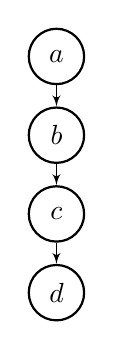
\begin{tikzpicture}
        [
        vertex/.style={circle,thick,draw,minimum size=2em},
        edge/.style={->,> = latex'}
        ]
    \node[vertex] (1) at (0,3) {$a$};
    \node[vertex] (2) at (0,2) {$b$};
    \node[vertex] (3) at (0,1) {$c$};
    \node[vertex] (4) at (0,0) {$d$};
    \draw[edge] (1) -- (2);
    \draw[edge] (2) -- (3);
    \draw[edge] (3) -- (4);
    \end{tikzpicture}
    \caption{Graph representation of $\poset{L}$ from Example~\ref{example:posetl}.}
    \label{figure:posetl}
\end{figure}

A partial order that is also total is called a \emph{linear order}; every pair of elements are comparable in a linear order. Note that the graph describing a linear order is a path graph. For simplicity, we represent a linear order in string form. For Example~\ref{example:posetl}, we write \lin{abcd}.

For a poset $\poset{P}$, a linear order $\poset{L}$ that extends $\poset{P}$ is called a \emph{linear extension} or \emph{linearization} of $\poset{P}$, and we write $\poset{P} \lext \poset{L}$ iff $\poset{L}$ is a linearization of $\poset{P}$. For example, for $\poset{P}$ from Example~\ref{example:posetp} and $\poset{L}$ from Example~\ref{example:posetl}, $\poset{P} \lext \poset{L}$. Note that a linearization of a poset is equivalent to a topological sort of the graph describing that poset.

The set of all linearizations of $\poset{P}$ is denoted $\lang{\poset{P}}$. We shall consider it the \emph{language} of a poset. For $\poset{P}$ from Example~\ref{example:posetp}, $\lang{\poset{P}} = \set{\lin{abcd},\lin{acbd}}$. For $\poset{L}$ from Example~\ref{example:posetl}, $\lang{\poset{L}} = \set{\lin{abcd}}$.

Now, we are ready to give the definition of \emph{Poset Cover Problem}.

% definition:pcp
\begin{definition}[Poset Cover Problem]
    Given a set of linear orders $\Upsilon$, find a set of partial orders $C$, called a cover, such that $\abs{C}$ is minimal and $\Upsilon = \bigcup_{\poset{P} \in C} \lang{\poset{P}}$.
    \label{definition:pcp}
\end{definition}

% example:cover example
\begin{example}
    Given the set of linear orders $\set{\lin{abfce},\lin{bafce},\lin{abcfe},\lin{abfec}}$ over $\set{a,b,c,f,e}$, a minimal poset cover of two posets $\poset{A},\poset{B}$ is shown in Figure~\ref{figure:cover example c} with ${\lang{\poset{A}} = \set{\lin{abfce},\lin{abcfe},\lin{abfec}}}$ and ${\lang{\poset{B}} = \set{\lin{bafce}}}$.
    \label{example:cover example}
\end{example}

% figure:cover example
\begin{figure}
    % figure:cover example c
    \begin{subfigure}[b]{0.5\textwidth}
        \centering
        \begin{subfigure}[b]{0.4\textwidth}
            \centering
            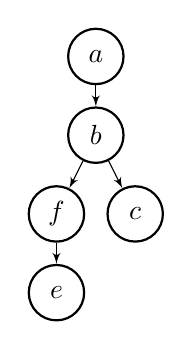
\begin{tikzpicture}
                [
                vertex/.style={circle,thick,draw,minimum size=2em},
                edge/.style={->,> = latex'}
                ]
            \node[vertex] (1) at (1,4) {$a$};
            \node[vertex] (2) at (1,3) {$b$};
            \node[vertex] (3) at (0.5,2) {$f$};
            \node[vertex] (4) at (0.5,1) {$e$};
            \node[vertex] (5) at (1.5,2) {$c$};
            \draw[edge] (1) -- (2);
            \draw[edge] (2) -- (3);
            \draw[edge] (3) -- (4);
            \draw[edge] (2) -- (5);
            \end{tikzpicture}
            \caption*{Poset $\poset{A}$}
        \end{subfigure}%
        \begin{subfigure}[b]{0.4\textwidth}
            \centering
            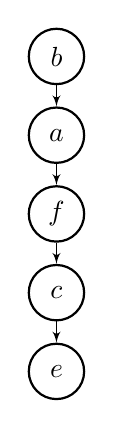
\begin{tikzpicture}
                [
                vertex/.style={circle,thick,draw,minimum size=2em},
                edge/.style={->,> = latex'}
                ]
            \node[vertex] (6) at (4,4) {$b$};
            \node[vertex] (7) at (4,3) {$a$};
            \node[vertex] (8) at (4,2) {$f$};
            \node[vertex] (9) at (4,1) {$c$};
            \node[vertex] (10) at (4,0) {$e$};
            \draw[edge] (6) -- (7);
            \draw[edge] (7) -- (8);
            \draw[edge] (8) -- (9);
            \draw[edge] (9) -- (10);
            \end{tikzpicture}
            \caption*{Poset $\poset{B}$}
        \end{subfigure}
        \caption{A minimal cover.}
        \label{figure:cover example c}
    \end{subfigure}%
    % figure:cover example c'
    \begin{subfigure}[b]{0.5\textwidth}
        \centering
        \begin{subfigure}[b]{0.4\textwidth}
            \centering
            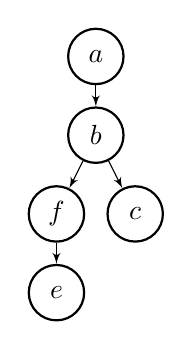
\begin{tikzpicture}
                [
                vertex/.style={circle,thick,draw,minimum size=2em},
                edge/.style={->,> = latex'}
                ]
            \node[vertex] (1) at (1,4) {$a$};
            \node[vertex] (2) at (1,3) {$b$};
            \node[vertex] (3) at (0.5,2) {$f$};
            \node[vertex] (4) at (0.5,1) {$e$};
            \node[vertex] (5) at (1.5,2) {$c$};
            \draw[edge] (1) -- (2);
            \draw[edge] (2) -- (3);
            \draw[edge] (3) -- (4);
            \draw[edge] (2) -- (5);
            \end{tikzpicture}
            \caption*{Poset $\poset{C}$}
        \end{subfigure}%
        \begin{subfigure}[b]{0.4\textwidth}
            \centering
            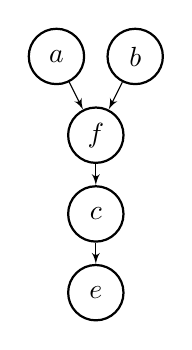
\begin{tikzpicture}
                [
                vertex/.style={circle,thick,draw,minimum size=2em},
                edge/.style={->,> = latex'}
                ]
            \node[vertex] (6) at (3.5,4) {$a$};
            \node[vertex] (7) at (4.5,4) {$b$};
            \node[vertex] (8) at (4,3) {$f$};
            \node[vertex] (9) at (4,2) {$c$};
            \node[vertex] (10) at (4,1) {$e$};
            \draw[edge] (6) -- (8);
            \draw[edge] (7) -- (8);
            \draw[edge] (8) -- (9);
            \draw[edge] (9) -- (10);
            \end{tikzpicture}
            \caption*{Poset $\poset{D}$}
        \end{subfigure}
        \caption{Another minimal cover.}
        \label{figure:cover example c'}
    \end{subfigure}
    \caption{Minimal covers for the set $\set{\lin{abfce},\lin{bafce},\lin{abcfe},\lin{abfec}}$.}
    \label{figure:cover example}
\end{figure}

A minimal poset cover may not be unique and the languages of the posets in a cover may overlap. For Example~\ref{example:cover example}, there is another minimal poset cover, shown in Figure~\ref{figure:cover example c'}, with overlapping languages ${\lang{\poset{C}} = \set{\lin{abfce},\lin{abcfe},\lin{abfec}}}$ and ${\lang{\poset{D}} = \set{\lin{abfce},\lin{bafce}}}$.

\section{Swap Graph}
% NOTE: re-write a better intro
*Since the poset cover problem is proved to be NP-complete, we decided to utilize the power of SAT solvers. However, a naive encoding would easily result in superpolynomial reduction. An efficient encoding requires some preprocessing using notions introduced as follows.

% put naive here?

The \emph{swap} relation $\swap$ describes the case of ``off by one swap'' between linear orders with shared universe: for linear orders $\poset{L}_1$~and~$\poset{L}_2$, $\poset{L}_1~\swap~\poset{L}_2$ iff there are $x, y \in \uni$ such that $\leq[\poset{L}_1] \cap \leq[\poset{L}_2] = {(\leq[\poset{L}_1] \cup \leq[\poset{L}_2])} - \set{(x,y),(y,x)}$; to specify which $x,y$ induce* the relation, we write $\swap[x,y]$. For example, \lin{abcd} $\swap[b,c]$ \lin{acbd}. Note that $\swap$ is symmetric.

For a set of linear orders $\Upsilon$, the \emph{swap graph} $\sgraph{\Upsilon}$ of it is the undirected graph $\tuple{V,E} = \tuple{\Upsilon,\swap}$. Figure~\ref{figure:graphlp} shows the swap graph $\sgraph{\lang{\poset{P}}}$ for $\poset{P}$ from Example~\ref{example:posetp}. Note that a swap graph built from the language of a poset is connected.

% figure:graphlp
\begin{figure}
    \centering
    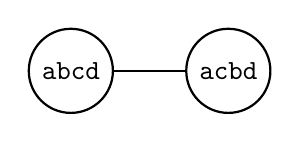
\begin{tikzpicture}
        [
        vertex/.style={circle,thick,draw,minimum size=2em},
        edge/.style={thick}
        ]
    \node[vertex] (1) at (0,0) {\lin{abcd}};
    \node[vertex] (2) at (2,0) {\lin{acbd}};
    \draw[edge] (1) -- (2);
    \end{tikzpicture}
    \caption{Swap graph $\sgraph{\lang{\poset{P}}}$ for $\poset{P}$ from Example~\ref{example:posetp}.}
    \label{figure:graphlp}
\end{figure}

% put encoding here
% NOTE what we'll arrive at ? what do we get out of it ?
*Now we reduce the poset cover problem to SAT. To find the minimal cover, we query SAT solver with increasing number of posets in our cover, starting from 1.

% prop var
Let $C$ denote the cover. For all posets $\poset{P} \in C$ and $x \neq y \in \uni$, we encode as $\satvar{x,y}{\poset{P}}$ the case that $x \leq[\poset{P}] y$.

% poset_cover.py : poset_axioms
First off, for the poset axioms, we encode antisymmetry as
$$
\bigwedge_{\poset{P} \in C} \bigwedge_{x \neq y \in \uni} \neg (\satvar{x,y}{\poset{P}} \wedge \satvar{y,x}{\poset{P}})
$$
and transitivity as
$$
\bigwedge_{\poset{P} \in C} \bigwedge_{x \neq y \neq z \in \uni}
\satvar{x,y}{\poset{P}} \wedge \satvar{y,z}{\poset{P}} \implies \satvar{x,z}{\poset{P}}
$$
and omit reflexivity for simplicity*.

% NOTE this is bad bad bad. must do bettter
*The poset cover problem can now be restated in logical formulae.

Let $\Upsilon$ denote the input set of linear orders. We encode its solution constraints, $\Upsilon = \bigcup_{\poset{P} \in C} \lang{\poset{P}}$, in a twofold manner, by separately encoding $\Upsilon \subseteq \bigcup_{\poset{P} \in C} \lang{\poset{P}}$ and $\Upsilon \supseteq \bigcup_{\poset{P} \in C} \lang{\poset{P}}$.

% poset_cover.py : le_constraints
For $\Upsilon \subseteq \bigcup_{\poset{P} \in C} \lang{\poset{P}}$, it effectively states that for all $\poset{L} \in \Upsilon$, there is some $\poset{P} \in C$ such that $\poset{P} \lext \poset{L}$. We encode it as
$$
\bigwedge_{\poset{L} \in \Upsilon} \bigvee_{\poset{P} \in C} \bigwedge_{x,y \in \complmt{\leq[\poset{L}]}} \neg \mathtt{P}_{x,y}^{\poset{P}}
$$
by interpreting $\lext$ in its contrapositive form*.

For $\Upsilon \supseteq \bigcup_{\poset{P} \in C} \lang{\poset{P}}$, conversely, it states that for all $\poset{L} \not\in \Upsilon$, for all $\poset{P} \in C$, $\poset{P} \not\lext \poset{L}$. A naive encoding such as
$$
\bigwedge_{\poset{L} \in \complmt{\Upsilon}} \bigwedge_{\poset{P} \in C} \neg \bigwedge_{x,y \in \complmt{\leq[\poset{L}]}} \neg \mathtt{P}_{x,y}^{\poset{P}}
$$
would result in factorial blow-up as all the absent permutations* $\abs{\complmt{\Upsilon}} \in \bigo{\abs{\uni}! - \abs{\Upsilon}}$. However, we can exploit the property that a swap graph of poset language is connected to avoid this, by ``insulating'' each connected component $\upsilon \subseteq \Upsilon$ with a \emph{barrier}* set $bar(\upsilon) = \set{\poset{L} \in (\Upsilon - \upsilon) \mid \text{there is } \poset{L}' \in \upsilon \text{ s.t. } \poset{L}' \swap \poset{L}}$ and encoding the constraint as
$$
\bigwedge_{\upsilon \in comp(\Upsilon)} \bigwedge_{\poset{L} \in bar(\upsilon)} \bigwedge_{\poset{P} \in C} \neg \bigwedge_{x,y \in \complmt{\leq[\poset{L}]}} \neg \mathtt{P}_{x,y}^{\poset{P}}
$$
where $comp(\Upsilon)$ is the family of all connected components in $\Upsilon$.

% whats a proposition?
% should i be like: given xxx yyy and such that ...
% should i draw an image illustrating barriers?
\begin{proposition}
    Barrier encoding entails naive encoding; that is,
    \begin{align*}
        & \forall_{\upsilon \in comp(\Upsilon)} \forall_{\poset{L} \in bar(\upsilon)} \forall_{\poset{P} \in C} \poset{P} \not\lext \poset{L}\\
        \models & \forall_{\poset{L} \not\in \Upsilon} \forall_{\poset{P} \in C} \poset{P} \not\lext \poset{L}
    \end{align*}
\end{proposition}
\begin{proof}
    We shall give a simple proof by contradiction. Suppose barrier encoding holds. Suppose naive encoding does not hold. Then there are some $\poset{L} \not\in \Upsilon$ and $\poset{P} \in C$ such that $\poset{P} \lext \poset{L}$. Per assumption, $\poset{L} \not\in bar(\upsilon)$ for all components $\upsilon$, but then $\sgraph{\lang{\poset{P}}}$ is not connected, a contradiction.
\end{proof}

% put new encoding here?
Barrier encoding is polynomial in the size of $\Upsilon$ since $\abs{bar(\upsilon)} \in \bigo{\abs{\upsilon} \times \abs{\uni}}$ for all $\upsilon$.

% where to put sat iff proof?
How do I do this part exactly? It's true by def?

%########################################

\section{Problem Definition?or Poset covered Problem}
intro pcp; intro converse of lin; intro trivial non-max solution? intro np completeness?

The poset covered problem is: given a set of linearizations $\Upsilon$, find a set of posets $\mathcal{C}$, called a covered, such that $\Upsilon = \bigcup_{P \in C} \mathcal{L}(P)$ and that $|\mathcal{C}|$ is minimal.

\begin{theorem}
    insulating barrier method where?
\end{theorem}

\section{SAT Encoding Part}
We use the boolean logic of z3 SMT solver from MS research. Since poset is connected, by contraposition, we can first divide and conquer on connected components of the swap graph, by solving each component individually.

We then check with incrementing number of posets to find the minimal number of posets to covered each component. We first encode the axioms of posets; namely, reflexivity, antisymmetry, and transitivity. Next, we encode the extension constraint with contraposition from input linearizations to reduce the number of variables. Finally, we encode the non-extension constraint with negation of extension constraint on the insulating barrier.

\section{Exp Part}
NOTE: how do i put graph here?

\section{Conclusions}

\section{References}
NOTE: how to use list?

\section{Appendix}

\begin{theorem}
    Permutations and Nerode
\end{theorem}

\begin{theorem}
    (Corollary of Szpilrajn extension theorem) For a partial order $\leq$, $\leq = \bigcap_{< \in \mathcal{E}(\leq)} <$.
\end{theorem}

\begin{theorem}
    (Heath and Nema) If $x \incomp y$ for $\leq$ and there is $< \in \mathcal{E}(\leq)$ such that $x \covered y$ for $<$, then there is $<' \in \mathcal{E}(\leq)$ such that $y \covered x$ for $<'$.
\end{theorem}

\begin{theorem}
    Swap graphs are connected by Kendall tau paths
\end{theorem}

\begin{theorem}
    %(Szpilrajn Theorem) For a partial order $\poset{P}$, there exists a linear order $\mathcal{L}$ that extends $\poset{P}$; that is, $\leq_{\poset{P}} \subseteq \leq_{\mathcal{L}}$.
    \label{theorem:szpilrajn}
\end{theorem}

\begin{theorem}
    (Pruesse? and Ruskey) For a poset $\poset{P}$, the swap graph $\mathcal{G}(\poset{P})$ is connected. cite???
\end{theorem}

That's it? should we move the swap things to motivations?

\end{document}
